% Thesis!

% Two Column Format
\documentclass[11pt]{article}
%this allows us to specify sections to be single or multi column so that things like title page and table of contents are single column
\usepackage{multicol, caption}
\usepackage{verbatim}

\usepackage{setspace}
\usepackage{url}

\usepackage{graphicx}

%%% PAGE DIMENSIONS
\usepackage{geometry} % to change the page dimensions
\geometry{letterpaper}

\setcounter{secnumdepth}{5}

\graphicspath{ {./images/} }

\newenvironment{Figure}
  {\par\medskip\noindent\minipage{\linewidth}}
  {\endminipage\par\medskip}

\begin{document}

%%%%%%%%%%%%%%%%%%
%%% Cover Page %%%
%%%%%%%%%%%%%%%%%%

\title{\vfill A Testing Framework for Web Application} %\vfill gives us the black space at the top of the page
\author{
By Taggart Ashby \vspace{10pt} \\
}

\maketitle

\vfill  %in combination with \newpage this forces the abstract to the bottom of the page

%%%%%%%%%%%%%%%%
%%% Abstract 
%%% VERY General overview of problem and solution in paper
%%%%%%%%%%%%%%%%
\begin{abstract}
Our framework is the best framework because we made it and we're awesome.
\end{abstract}

\thispagestyle{empty} %remove page number from title page
\newpage

%end the 1 column format

%start 2 column format
\begin{multicols}{2}
%Start numbering first page of content as page 1
\setcounter{page}{1}

%%%%%%%%%%%%%%%%%%%%
%%% Introduction/Motivation
%%% More detailed, but still general, description of problem and why we want to solve it
%%%%%%%%%%%%%%%%%%%%
\section{Introduction}
Since the advent of the internet, the web has undergone an impressive evolution from plain-text webpages to the highly stylized and functional pages that we see today. In the last four to six years there has been an explosion of new web technologies that make applications more functional: HTML5, CSS3, WebGL, Touch APIs, Geo-location, and a host of others. \cite{EvolutionOfWeb} In that same time period, the number of global internet users has grown to somewhere around 2.5 billion people. \cite{EvolutionOfWeb} The combination of these new technologies and the ever-increasing usage of the internet has led to a significant growth in the number and complexity of web applications.
Like any piece of software, these web applications ought to be tested in order to determine their correctness and give their users the best experience possible. Unfortunately, web applications are the new kids on the block and there is very little conventional wisdom on how to test them. Their dynamic nature and network communication require a different testing toolkit than their predecessors. In addition, web applications are being produced at an incredible rate and so there's often little time to test.
We can see that this is not a solved problem by looking at some of the biggest web application around. A 2011 study showed that YouTube has at least eight errors, Apple has at least seven, Microsoft at least four, and the list goes on. \cite{ErrorsInTheWild} That may seem like a incredibly small amount for such monoliths, and, honestly, it is fairly small, but those are still errors in the software that ought to be fixed.
What this all boils down to is that there needs to be a framework in place for testing these multi-layer, multi-faceted web applications that is easy to use, quick to develop on, and thorough in its coverage. 

%%%%%%%%%%%%%%%%%%
%%% Background 
%%% Information needed for reader to know what’s going on
%%% 	Server/Client Communication
%%% 	Cloud services
%%% 	Appropriate terms and definitions
%%%%%%%%%%%%%%%%%%
\section{Background}
In an effort to make the rest of the paper more understandable and to define the terms used in the remainder of the paper, it is useful to have a section pertaining to the different concepts and technologies surrounding the web.
If one is familiar with HTML5, JavaScript, and Testing concepts and statistics, it will likely be safe to skip this background section.

\subsection{Web Application Strengths}
Web applications are great for both developers and consumers. They have a number of characteristics that make them more desirable than shrink-wrap software. These attributes are versioning, availability, platform independence, and the ability to rapidly prototype.

\subsubsection{Versioning}
Web applications can be updated at any time with instant roll-out and feedback. It requires absolutely no user interaction because the web page always serves the latest resources. In comparison to something like an operating system that requires users to manually update, this feature leads to applications that can address problems quickly, roll-out security updates instantly, and incorporate consumer feedback much more quickly than any other type of software. Another perk is that users are not given a choice. This can lead to occasional customer outrage, but more often than not it's a powerful gain for both feature improvement and application security.

\subsubsection{Availability}
Web application are available anywhere there's internet. No need to install anything on a given device most of the time. Due to the ever-increasing popularity of mobile devices, most applications have both mobile and full versions of their software and so the application is ``with you'' all the time.

\subsubsection{Multi-platform}
Very similar to the availability strength, web applications are platform independent. Whether you're on your phone, tablet, laptop, or PC, the application only requires a web browser with certain functionality and in this day and age all devices come equipped with browsers that should have no problems.

\subsubsection{Rapid Prototyping}
Web applications are fantastic for rapid prototyping because of all of the strengths discussed above. An idea can be prototyped and posted on a website quickly and rapid iteration can occur without the user even necessarily noticing. There are a number of web tools that will outline where users are clicking, what features they're using, how long they're spending on a given page or step of a process, and a number of other metrics that can make iterations more directed and effective.


\subsection{Web Features}
Here I'll discuss some of the prevalent technologies that recently appeared in web applications and development. By no means is this an exhaustive list, just a sampling of the more prominent ones.

\subsubsection{HTML5}
The latest revision of HTML is HTML5 which first debuted on Firefox back in 2009. \cite{EvolutionOfWeb} HTML5 has not been officially recommended by the W3C (World Wide Web Consortium) who is the official keeper and recommender of web standards, however, there is a plan for final recommendation this year, 2014, called Plan 2014. \cite{Plan2014} What this means is that in 2014 the W3C will release a stable HTML5 Recommendation which will make HTML5 an official standard and help universalize all the separate implementations.
HTML5 brings a number of new features including: audio and video tags, the canvas element, drag-and-drop functionality, web storage, offline page support, and a number of other modern web features. A lot of HTML5's features revolve around the inclusion of multimedia in web pages and stronger graphical processing and programming.

\subsubsection{JavaScript}
JavaScript, though not the only scripting language with web use, is the primary language used to compliment HTML when making web applications. It is an interpreted language that is most often associated with client-side functionality, but in recent times has extended to the server-side. JavaScript is a prototype based object oriented scripting language with dynamic typing and first-class functions. Much of JavaScript's popularity stems from this dynamic nature that allows for quick, and often dirty, implementation of features in an often iterative environment.

\subsubsection{Node.JS}
Node.JS, often called simply Node, is a JavaScript API for creating and running servers. ``Node's goal is to provide an easy way to build scalable network programs.'' \cite{Node} Node was created in 2009 and is sponsored by Joyent. Node does not use thread-based networking, instead opting for a single-threaded event loop and non-blocking I/O. Node allows developers to create and control web servers without the need for external software, such as Apache, commonly found in other sites.
Node is found in a number of popular sites including: PayPal, The New York Times, Yahoo!, Uber, LinkedIn, Microsoft Azure, and a number of others. \cite{Node}
 
\subsection{Why Testing is Important}
I'm consistently surprised by how few people take testing seriously when it comes to non-trivial applications. 

\subsubsection{What is testing?}
IEEE defines software testing as ``the process of analyzing a software item to detect the differences between existing and required conditions (that is, bugs) and to evaluate the features of a software item.'' \cite{TestingDefinition}
Although there are a number of different types of tests and testing concepts, we will focus on Unit Testing and Continuous Integration.

\paragraph{Unit Testing}
Unit testing is the testing of specific functions and functionality. Generally this means the testing of individual functions but can extend to a set of functions that produce a single module of functionality. What's important to remember in regards to unit testing is that it tests just one portion of the code or system rather than interactions between modules or the entire system.

\paragraph{Continuous Integration}
Continuous integration, in the context of testing, is the term for a piece of software or service that continually runs tests on your code as you develop. The purpose of this is to make sure that new code is not breaking old tests and that new code is passing any tests you've written for it.
One of the most important pieces of this is that it is automatic. There should be no need for a developer to do anything besides ``turn it on'' and start coding. As soon as a tool requires more than one or two interactions, it becomes much more of a nuisance and less of a helper.

\subsubsection{Testing Statistics}
It is widely accepted that the earlier a developer detects a defect, the easier it is to fix that defect. A famous book, ``Code Complete'' by Steve McConnell \cite{DefectPic}, includes the following figure, showing this statistic on a rough graph.

\begin{Figure}
	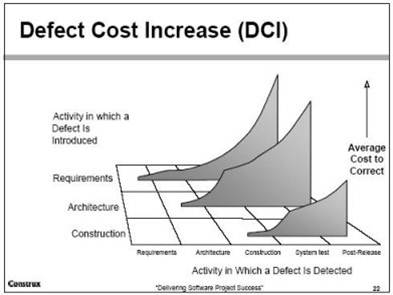
\includegraphics[width=\linewidth]{defectcost.jpg} 
	\captionof{figure}{\cite{DefectPic}}
\end{Figure}


\subsection{Client/Server Architecture}



%%%%%%%%%%%%%%%%%%%%%%%%%
%%% Product 
%%% User Manual
%%% 	Tools (programs, IDEs, scripts)
%%% 	Setup instructions
%%% 	Usage
%%%%%%%%%%%%%%%%%%%%%%%%%
\section{Product}


%%%%%%%%%%%%%%%%%%%%%%
%%% Implementation 
%%% 	Why I chose the tools I chose
%%% 	Scripts written to help out 
%%%%%%%%%%%%%%%%%%%%%%
\section{Implementation}


%%%%%%%%%%%%%%%%%%
%%% Evaluation
%%% PX Intro
%%%	Outline test suites
%%% PX Test metrics/results
%%%%%%%%%%%%%%%%%%
\section{Evaluation}



%%%%%%%%%%%%%%%%%%%%
%%% Related Work 
%%% Similar testing frameworks
%%% 	Why they're not as good as ours
%%%%%%%%%%%%%%%%%%%%
\section{Related Work}


%%%%%%%%%%%%%%%%%%
%%% Conclusion 
%%% Summary of what they just read
%%% Recap results
%%%%%%%%%%%%%%%%%%
\section{Conclusion}


%%%%%%%%%%%%%%%%%%%
%%% Future Work 
%%% Anything we wanted to do but didn't have time to
%%%%%%%%%%%%%%%%%%%
\section{Future Work}


%%%%%%%%%%%%%%%%%
%%% Appendices
%%% Actual Test Code
%%% Anything that needs an appendix
%%%%%%%%%%%%%%%%%
\section{Appendices}

\end{multicols}
\newpage

\bibliographystyle{IEEEannot}

\bibliography{paper}

\nocite{*}

\end{document}
